\documentclass[main.tex]{subfiles}
\begin{document}
\section{Architectural Choices}
% Architectural choices
% • How did they get data?
% • How do their components map to the architecture choice in the different tiers?

\todoL{It is not clear why we made certain choices}
\todoL{It is not clear what choices we made}

The architecture of the system is shown on figure \ref{fig:architecture}. The blue boxes represent Docker containers running. These are currently all running on the same physical machine -- the Docker Host in the diagram -- but ideally the services hosted in the docker containers would be hosted on multiple physical computers as the benefits of distribution are lost when distribution is not present. 

The web server runs on a separate host from the docker cluster and communicate with it through Local Area Network (LAN). The web server queries the Drill service, which in turn accesses the HDFS. The web server is accessed by a web client that may be running on a third host. This ensures that the Drill service itself acts as a data layer and is encapsulated and exposed through the web server.

The spark submission service is not shown on the diagram on figure \ref{fig:architecture} as it is not permanently running. It is only running for a limited period of time when submission of a spark job has been issued to the YARN cluster. It may even be killed before the end of the spark job without affecting the spark job because the spark job is submitted in cluster mode. The spark job will continue running on the YARN cluster and the output is written to the HDFS nodes, and the logs are written to the history server.

\begin{figure}[h]
    \centering
    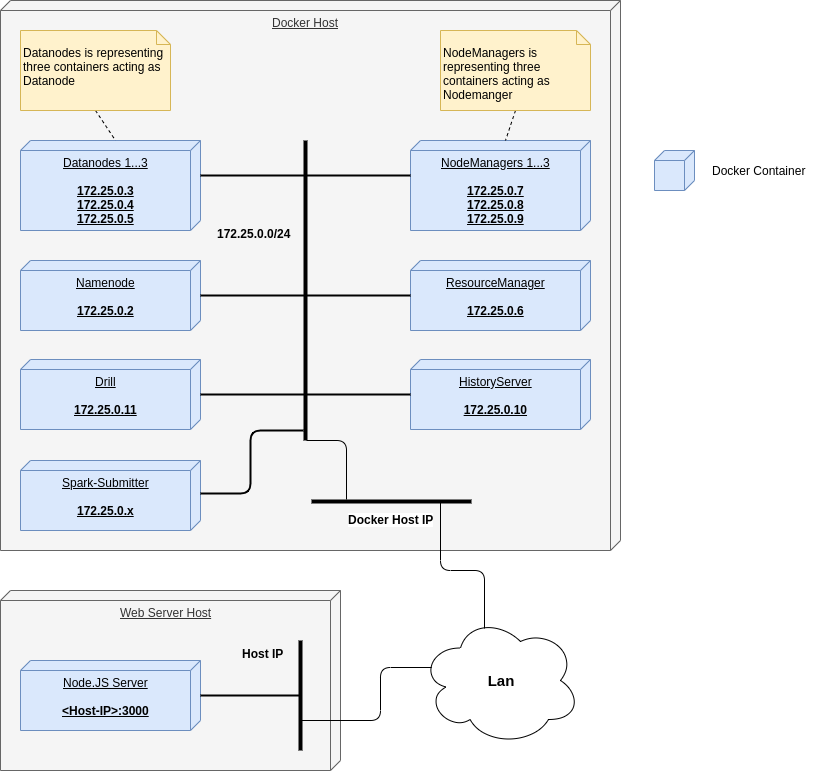
\includegraphics{Images/Cluster.png}
    \caption{The architecture of the system}
    \label{fig:architecture}
\end{figure}


\subsection{Cluster Managers}
Three of the major cluster managers that have been assessed are Spark standalone, YARN and Mesos \cite{clusterManagers}.
These three mentioned cluster managers are all very powerful with many sophisticated features. Each manager has its own strengths which must be considered when deciding upon which of the managers to be utilized in a project. 

\todoL{"Currently, the standalone mode does not support cluster mode for Python applications." - http://spark.apache.org/docs/latest/submitting-applications.html}

\paragraph{General}
The three managers have many common properties, however some differences are highlighted here. The operating systems they can be run on varies. Spark standalone is able to be run on the three major operating systems: MacOS, Windows and Linux. Mesos on the other hand is not able to run on Windows, but only Linux and MacOS. YARN runs on Linux and Windows, but not MacOS. This project utilizes docker containers which makes a shared Linux kernel available, so all three managers are able to be run.

YARN has the advantage over Spark standalone in being a general purpose cluster that can run a variety of jobs e.g. Spark, MapReduce and Storm. The standalone cluster is only able to run Spark jobs which makes less utilization of hardware resources. Mesos is in contrast to YARN also a general purpose cluster but the main difference is at the abstraction level. Mesos is able to share hardware resources for even more applications but also more complex to setup.



\textbf{Scheduling}
Spark uses a FIFO queue for scheduling applications, where each application uses all of the resources available on the cluster by default. The number of nodes can be limited per application and other resources are configured within the application. Mesos has a master-slave setup where the master releases resources which the slaves can accept or decline. This means that claiming resources and running jobs is up to the application. YARN utilizes a resource manager which is responsible for accepting job submissions and initializing an application specific ApplicationsMaster with the amount of requested resources. 

\textbf{Monitoring}
YARN, Mesos and Spark provide a web UI for detailed metrics and information regarding the status of the cluster and the applications that are running on the nodes. The three managers are very similar regarding this characteristic, however, Spark supplies a separate UI for each application. 

\end{document}